\newpage
\section{Ergebnis \& Handlungsempfehlung}\label{hauptabschnitt_5}
\subsection{Ergebnis}\label{hauptabschnitt_5_1}
Ein Trend zum Omni-Channel-Marketing ist erkennbar. Die Investitionen von Einzelhändlern sind mittlerweile digital getrieben und werden nach und nach auf Omni-Channel-Strategien ausgerichtet. Die Unternehmen werden in Zukunft bereit sein, aus jeder Geschäftsmöglichkeit das Beste herauszuholen, da die Kundenanforderungen sich verstärkt zum Onlinekauf weiterentwickelt haben und der Trend zu einem personalisierten Einkaufserlebnis führt.
\newline

Omni-Channel bedeutet dabei nicht nur Technologie, sondern hat auch Auswirkungen auf Prozesse und Organisationen. Die Rationalisierung und Veränderung der Kernprozesse rund um Bestellung, Abholung, Lieferung und Rückgabe bedeutet für Unternehmen die Einbeziehung von Kanälen, Logistik, Lieferdiensten, Lagerverfügbarkeit und Mitarbeitern.
\newline

In diesem Szenario wollen Einzelhändler ihren Kunden und Kundinnen mehr Flexibilität bei der Bezahlung, Abholung, Lieferung, Erstattung und Rückgabe bieten. Dies ist ein skalierbarer Prozess für alle Geschäfte, Marken und Länder.
Um die Kundenbedürfnisse zu befriedigen, werden Händler daher mittelfristig eine Lösung suchen, die alle Hauptakteure im Bestellfluss (Geschäfte, Handel, Kundendienst und Verantwortlichkeit) mit einem einzigartigen System für das Bestellmanagement verbindet.


BABOR ist die Entwicklung zum Online-Geschäft und damit einhergehend auch die Umsetzung verschiedener Omni-Channel-Ansätze gelungen. BABOR konnte die Umsätze durch den Online-Handel nicht nur deutlich verbessern, auch global gesehen hat die Marke an Bekanntheit und Kundenzuwachs gewonnen. Für einen neuen Logistik- und Produktionsstandort, der weiterhin in Aachen sein wird, hat BABOR 2021 60 Millionen Euro investiert und möchte diesen bis 2024 fertigstellen. Dabei wird weiterhin daran gearbeitet, noch nachhaltiger, aber auch schneller zu produzieren und bei der Logistikabwicklung schlankere Prozesse zu erreichen. BABOR bietet seinen Kosmetikpartnern an, Logistikprozesse bei Online-Käufen zu übernehmen und zahlt dafür eine Provision aus.
\newline

Ein Schlüssel zur Erhöhung der Umsätze von Beautyprodukten bei BABOR besteht darin, dass eine neue und moderne CRM-Software alle verfügbaren Daten, unter anderem über das eingeführte PIM-System, zusammenführt und somit erst eine ganzheitliche Sicht auf den Kunden oder Kundin ermöglicht wird. Durch die bessere Nachverfolgung des Kaufverhaltens und die Personalisierung von Kundenerfahrungen vor Ort, unabhängig davon, ob der Kauf in einem Kosmetikstudio, im Online-Shop oder im Ausland stattfindet, können die Umsätze  gesteigert werden.

\begin{figure}[!ht]
	\centering
	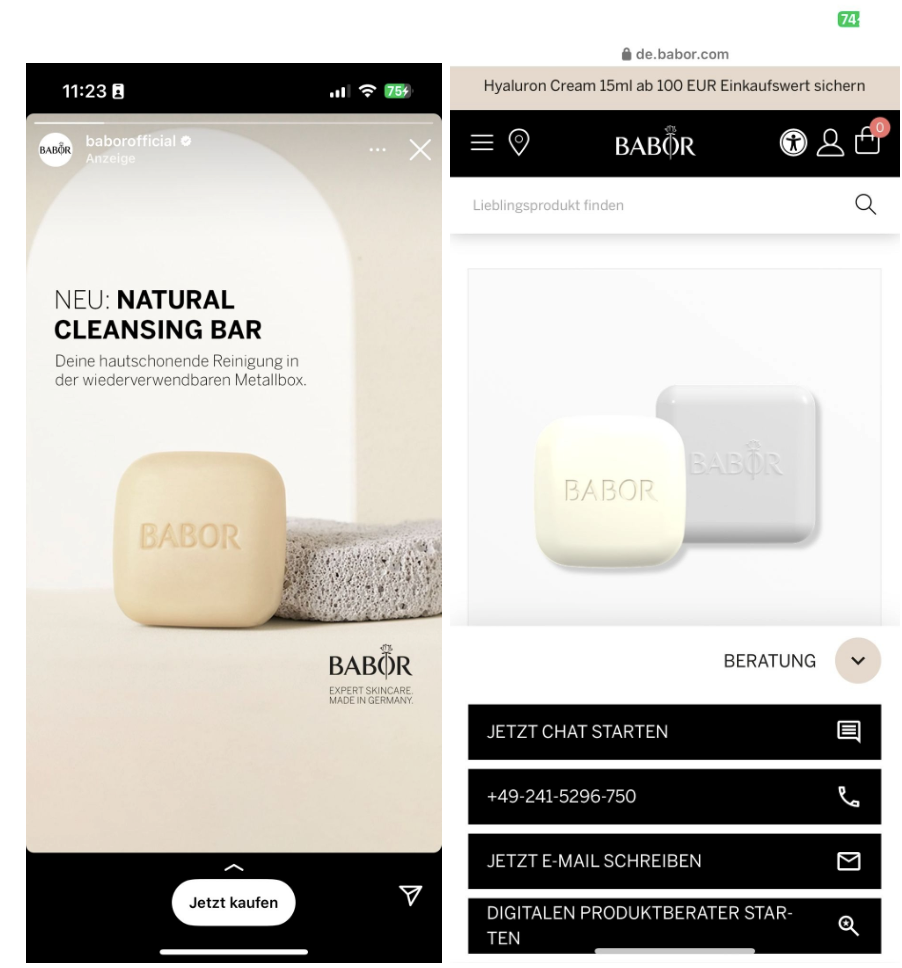
\includegraphics[width=0.7\textwidth]{src/abbildungen/babor_ad.png}
	\caption[Quelle: BABOR Webseite und Instagram AD]{Werbung über Social-Media und Auswahlmöglichkeiten zur Beratung, Quelle: ~\autocite[S.14]{babor2023}}
       \label{fig:Beschreibung}
\end{figure}

In den sozialen Medien versucht BABOR durch regelmäßige Postings, gezielte Werbung und gutes Marketing Aufmerksamkeit auf bestimmte Produkte zu generieren.
\newline
Für ein vorgeschlagenes Produkt wird zudem über den Online-Shop eine Beratung angeboten (z.B. über Telefon, E-Mail oder per Chat) und es kann auch eine eigens entwickelte Hautanalyse, also eine digitale Hautberatung, in Anspruch genommen werden, um das Einkaufserlebnis zu personalisieren und auf jeden Hauttypen empfohlene Produkte zu empfehlen. Zudem besteht die Möglichkeit, durch Cross Selling Produkte anzubieten, die durch das Personalisieren eine erhöhte Wahrscheinlichkeit mit der Übereinstimmung des Kunden oder der Kundin finden. Neukunden erhalten die Möglichkeit, einen Willkommensgutschein in Anspruch zu nehmen, wodurch ein Rabatt bei der ersten Bestellung entsteht. Zudem wird die Möglichkeit angeboten, einen Newsletter zu informieren, bei dem Kunden ihre E-Mail hinterlegen und in regelmäßigen Abständen zur Marke BABOR oder neuen Produkten News oder per E-Mail erhalten.
In der Regel werden zudem bei Bestellungen Gratisproben verteilt, um auf weitere Produkte aufmerksam zu machen.
\newline

Viele BABOR Produkte werden von den Konsumierenden auch über Marktplätze wie Amazon gekauft, weshalb auch BABOR dort sehr aktiv ist und mehrere Key Account Manager eingestellt hat, die sich nur um das Projekt Amazon kümmern. Dort wird zum Beispiel für bestimmte Suchbegriffe auch aktiv Werbung geschaltet, so dass BABOR Produkte in der Kategorie Kosmetik schnell und mit Priorisierung angezeigt werden.
\newline
Über Amazon ist es zum Beispiel möglich, neben den verschiedenen Zahlungsmethoden auch Abonnements für BABOR in verschiedenen Intervallen abzuschließen, so dass ein Produkt in regelmäßigen Abständen automatisch wieder geliefert wird. Zudem garantiert Amazon mit ihrem Prime Angebot eine Gratis Lieferung am nächsten Tag. Durch die große Anzahl an Kosmetikstudios in Deutschland hat sich BABOR deutschlandweit über 2000 Kosmetikpartner herausgesucht, so dass zusätzlich in der Nähe eine Produktberatung in Anspruch genommen werden kann oder Produkte gekauft werden können.
\newline

Bei dem B2B-Geschäft bietet BABOR an die Auftraggebenden weiter einen Fulfillment-Prozess an, bei dem der komplette Logistikprozess von BABOR abgewickelt werden kann.

\subsection{Handlungsempfehlung}\label{hauptabschnitt_5_2}
Unternehmen sollten eine Omni-Channel-Strategie einführen, wenn sie eine bessere Kundenerfahrung und eine höhere Kundenbindung anstreben. Dafür ist es sinnvoll, verschiedene Faktoren zu berücksichtigen.
Unternehmen sollten ihre Kunden und Kundinnen besser verstehen, um festzustellen, wie diese ihre Produkte und Dienstleistungen bevorzugen. Hierfür sollte zum Beispiel das Konzept der Customer Centricity durchgeführt werden, um einen Blick auf die Kundensicht zu erhalten.
\newline

Einige Kunden oder Kundinnen bevorzugen den Kauf über E-Commerce-Websites, andere bevorzugen den Kauf in Geschäften und wiederum andere bevorzugen den Kauf über mobile Apps. Eine Omni-Channel-Strategie ermöglicht es Unternehmen, alle diese Kanäle zu nutzen, um ihre Kunden zu bedienen. Wenn die Konkurrenz bereits eine Omni-Channel-Strategie implementiert hat, kann es sinnvoll sein, ebenfalls eine solche Strategie einzuführen, um wettbewerbsfähig zu bleiben. Eine Omni-Channel-Strategie kann dazu beitragen, dass das Unternehmen eine einheitliche Markendarstellung in allen Kanälen beibehält. Dies trägt dazu bei, die Stärkung des Markenimages herzustellen. Unternehmen sollten auch die Kosten-Nutzen-Analyse durchführen, um festzustellen, ob die Einführung einer Omni-Channel-Strategie für sie wirtschaftlich sinnvoll ist.
\newline

Automatisierung sollte in möglichst vielen Bereichen eingeführt werden, wo es Sinn macht. Beispiele sind immer wieder wiederholende Prozesse. Ein angebotener Self-Service an sich spart Kosten ein und erhöht die Flexibilität der Konsumierenden in den Kontaktpunkten. Die Kosten, die dabei im Self-Service gespart werden, können so in komplexere Themen investiert werden, wie zum Beispiel die Kundenzufriedenheit oder in das Expertenwissen, um auch dort die entsprechenden Kennzahlen optimieren zu können. Durch verbesserte Ausbildungsmöglichkeiten der Mitarbeiter steigt die Expertise in den Fachbereichen und so können schneller, kompetenter und einfacher Lösungen gefunden werden. Gleichzeitig ist es notwendig, verschiedene Kanäle im Kundenkontakt zu nutzen. Dies ist bei weitem noch nicht so verbreitet, wie man es erwarten würde.
\newline

Zudem sollte eine Zielgruppenanalyse  stattfinden, um zu einem Ergebnis zu kommen, welche Kanäle angeboten werden. Wenn das Zielklientel zum Beispiel 65+ ist, sollte das Thema Video-Chat in diesem Bereich nicht das präferierte Hauptziel sein, die Kundschaft anzusprechen. Dabei sollte analysiert werden,  was der Kunde oder die Kundin benötigt und welche Anforderungen gestellt werden.
Auch die Telefonie bleibt ein wichtiger Kanal im persönlichen Kundenkontakt. In diesem Bereich sollten Experten ausgebildet werden, um die Kundschaft erfolgreich und einfach beraten zu können.
\newline

Es gilt auch, Flexibilität in den Kontaktpunkten herzustellen. Die Kunden und Kundinnen wollen nicht permanent mit dem Unternehmen direkt kommunizieren müssen. Falls  jedoch Kommunikation von Seiten des Kunden oder der Kundin gewünscht wird, dann sollten sie die Flexibilität geboten bekommen, den Weg zu entscheiden und dabei schnelle und kompetente Hilfe angeboten bekommen. Im Optimalfall können diese Fragen durch ausgebildetes Expertenwissen beantwortet werden. Um bessere und genauere Entscheidungen treffen zu können, werden für den direkten Kundenkontakt für den Berater entsprechende Kundendaten bereitgestellt, die bei komplexen Themen im persönlichen Kundendialog unterstützen.
\newline

Omni-Channel-Strategien können Unternehmen dabei helfen, ihre Kunden und Kundinnen besser zu bedienen und ihre Kundenerfahrung zu verbessern. Die Einführung einer solchen Strategie erfordert jedoch eine sorgfältige Planung und Umsetzung, um sicherzustellen, dass sie den Bedürfnissen des Unternehmens und seiner Kunden entspricht.
